% Chapter Template

\chapter{Extending the Test Framework} % Main chapter title
\label{Chapter4}

%----------------------------------------------------------------------------------------
%	SECTION 1
%----------------------------------------------------------------------------------------

\begin{itemize}
    \item Modify test framework
    \item Modify fakeradio to output layout
    \item Get dual link types working
    \item Be able to define different WiFi layouts
    \item 
\end{itemize}


\begin{itemize}
    \item Currently, no way to easily determine what topology is in machine readable format
    \item What info is needed for this 
    \item How can we represent it?
    \item Why format?
    \item JSON vs CSV
\end{itemize}


%-----------------------------------
%   SECTION 1
%-----------------------------------
\section{Joint WiFi \& Radio Tests}
A key part of the test framework that was missing was support for networks with both WiFi and radio link types. 
This presents a major limitation  to the test framework as real Serval networks would feature both of these network links.
To implement this feature, several additions need to be made to the test framework.

First, the ability to define which link simulation will be used for each nodes needs to be defined.
This allows test definition writers to define the functionality(??) of each of the nodes. 
For instance, test writers are able to define if a specific node in a topology is using the fakeradio tool or simply acting as WiFi, or even, both. 

Next, the ability to define specific network topologies will need to be added.
This already exists in the case of the fakeradio networks as discussed in the previous chapters, this is not easily done with the simulated WiFi tool.

Once these two pieces of functionality have been added to the test framework, developers will be able to test considerably larger and more complicated network topologies with ease.
With this expanded test framework the Serval team will be able to significantly improve their knowledge of the Serval network; complicated, larger, and reproducible tests offer a huge benefit to the goals of the Serval team. \todo{rewrite, this is bad}

What needed to be done for this?
\begin{itemize}
    \item Add capability to define interface to use
    \item Strip definitions to get lists of what interfaces for each node
    \item For each node, add the interfaces that are in lists
    \item For each node, add appropriate configuration
    \item Pass LBARD rules to fakeradio as per normal
\end{itemize}

\todo{Mention that this is done in a NEW FILE}
\todo{Add new testdefs file}

To achieve this, several features need to be implemented. 
The first feature is defining the interfaces to be used on a per-node basis.
With this, nodes can each have their own configuration, allowing for some nodes to have WiFi enabled while others only have fakeradio interfaces.
Next, the ability to define WiFi topologies will need to be added, as currently it appears to only be possible to have nodes communicating with every other node without any defined topology.

To ensure that this does not affect pre-existing LBARD tests, two new files will be created.
The first is the \emph{topologies} test file.
This file is just a new test file that outlines the new tests to be implemented.
Further, since these will need 

\subsection{Defining interfaces per node}
\begin{itemize}
    \item \textbf{Explain original scenario}
    \item Pass n nodes, all are labelled as specified radio type
    \item n Serval interfaces and n LBARD interfaces are started
    \item fakeradio is started
    \item Test is run, communicate, log it all
    \item Limitation: as it is treating each node the same with no differentiation between, no way to enable wifi on some nodes and not others
\end{itemize}
\todo{briefly explain original scenario}

\todo{Explain why we need to enable interfaces}

The first step to completing this is to determine what nodes need which configuration applied.
Two possibilities exist for this; manually define the configurations for each node or automatically determine which configuration is required for each node.
Since each node that will be connected by fakeradio needs to be defined already, it was decided to use this information to determine what configuration the node needed.

Each test that uses fakeradio contains a string in the setup function defining the links between nodes.
An example of this is shown in \todo{add figure}. 
The string defines the links in the format "allow between [n],[m];" where n and m are the 0-indexed serval-dna instance number.
This is suitable to use since every node in a topology using fakeradio must be specified in this string, meaning that \emph{every} node that requires LBARD interfaces defined will be listed here.
As the WiFi functionality does not need to have the topology defined in such a way it is necessary to define a new string, simply listing the nodes that require WiFi to be enabled. 

These strings are passed to the \emph{start\_instances} function. 
To determine what nodes to enable the configurations on, the node information needs to be stripped from the string.

To achieve this, multiple alterations need to be run on the strings.
The first is removing newline characters and replacing them with spaces.
This ensures that multiple line fakeradio rules will not break the node parsing.
Next, a \emph{sed} command is run, replacing every character that is not a number with a space character, stripping all information that is not specifically the number of the node.
The \emph{tr} command is then run, removing extraneous space characters, so that the string is just the node numbers separated by a single space character.
Finally, each space character is replaced with the \emph{sed} command with a newline character.
This results in two string of the node numbers, with each node on a new line.
To use these in the rest of the program, these strings are converted to an array, one for WiFi and one for fakeradio nodes.

With this information, we can now programmatically determine which configurations need to be enabled on each nodes.
To implement this however, one more step is required.
A new array \emph{all\_nodes} is created that simply lists all of the nodes in the test.
This array simply contains the combined unique set of the WiFi and fakeradio arrays.

Next, the program iterates through the \emph{all\_nodes} array, and adds the string 'wifi', 'fakeradio' or 'wifi fakeradio' to an array of strings at the index of the node.
This results in an array where at the index of a given node the interfaces are textually listed.
\todo{add better explanation - diagram?}
The framework then iterates through each node specified and sends the array to the \emph{configure\_servald\_server} function.


The \emph{configure\_servald\_server} is called for each node before the instance is started, and as such each configuration is unique to each instance of servald.
This means that we can now add the required configuration for a node without affecting other nodes.
When the configure\_servald\_server function is called the program simply calls the \emph{add\_servald\_interface} function with the interfaces needed for that given node.
When this is called the program iterates through the supplied interfaces (ie. 'wifi', 'fakeradio', or 'fakeradio wifi') and for each interface configures the servald instance appropriately.
For fakeradio instances, the only configuration that needs to be set is enabling http (to connect to LBARD) and setting the username and password for LBARD.

With this completed, it is now possible to run WiFi and fakeradio nodes side-by-side, with the appropriate interfaces enabled based on the test definition.
However this method has a major limitation; it is not possible to have complicated WiFi topologies with this method since WiFi nodes have zero restriction around what other WiFi nodes they can communicate with.
This means that while networks such as \todo{figure a; A-r-B-w-C-r-D} work, any network such as \todo{figure b} will not work as there is no way to restrict node E from connecting to node C.



\subsection{Defining wifi topologies}
When expanding the test framework to handle the mixed topologies, it was planned to implement functionality to define WiFi network layouts in the same format as defining fakeradio networks, however it was suggested to instead define wifi interfaces using existing tools found in the Serval-DNA framework.
While this meant that topology tests would be not have a consistent method of defining network layouts between radio and WiFi nodes, it would however be consistent with Serval-DNA tests.

Using the method previously outlined in the previous section, WiFi nodes all default to using the same WiFi interface - thus creating a fully-connected WiFi mesh sub-network, leading to every WiFi node being connected. 
This can be seen in \figurename{ \ref{fig:networkWifi1}}.
Each WiFi interface is essentially a sub-network, with nodes within a specified interface only able to communicate with nodes within the same interface as themselves.
Thus, to define a complicated network topology it is necessary to restrict which interfaces WiFi nodes can communicate on.

\begin{figure}
    \begin{centering}
        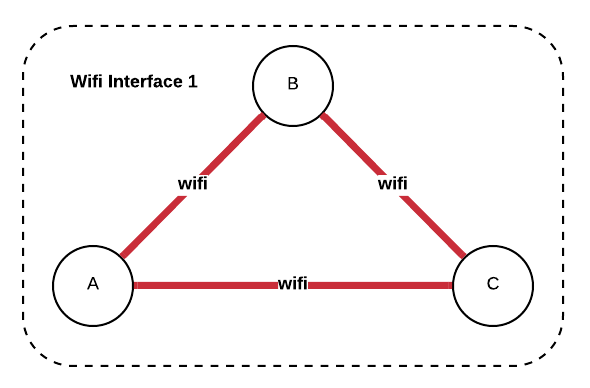
\includegraphics[width=14cm,height=20cm,keepaspectratio]{Figures/networkWifiInterface1.png}
        \caption{Network topology without defining interfaces}
        \label{fig:networkWifi1}
    \end{centering}
\end{figure}


In the Serval-DNA test framework, non- fully-connected WiFi networks are created by manually defining the WiFi interfaces that a specified servald interface is connected to.
To implement this, several changes need to be made.
The first is removing the functions added in the previous section that relate to WiFi.
This is because we'll no longer be defining WiFi nodes with a string passed to the setup functions.
Next, it was decided for every node to automatically have WiFi functionality enabled by default, but only connected to its own private interface. 
This is done by changing the configuration parsing added in the previous section to enable WiFi by default, but still only enabling LBARD as specified.

To connect nodes via WiFi they must now be connected to a specific WiFi interface as shown in \figurename{ \ref{fig:definingInterfaces}}.

\begin{figure}
    \begin{centering}
        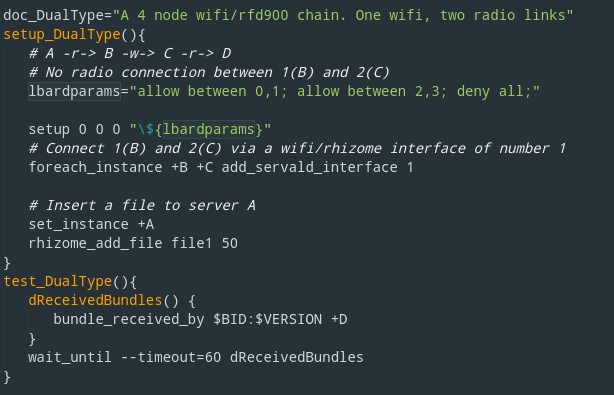
\includegraphics[width=14cm,height=20cm,keepaspectratio]{Figures/definingInterfaces.png}
        \caption{Defining WiFi interfaces}
        \label{fig:definingInterfaces}
    \end{centering}
\end{figure}

When a node is connected to multiple nodes at once, it will be able to communicate with all other nodes in those interfaces, while the connected nodes are still only able to communicate with nodes in the same interfaces as themselves.
This means that previously impossible network topologies such as WiFi chains can be implemented as shown in \figurename{ \ref{fig:networkWifi2}}.

\begin{figure}
    \begin{centering}
        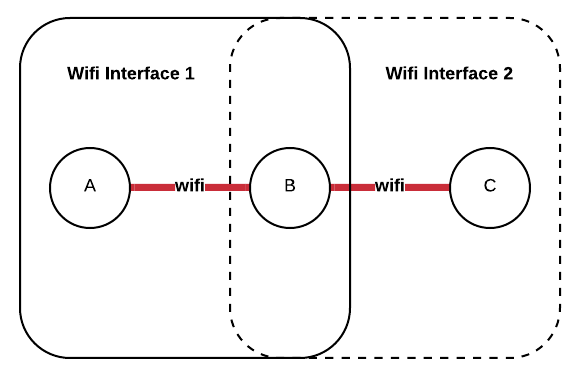
\includegraphics[width=14cm,height=20cm,keepaspectratio]{Figures/networkWifiInterface2.png}
        \caption{Network topology with two wifi interfaces defined}
        \label{fig:networkWifi2}
    \end{centering}
\end{figure}


\subsection{Adding utility functions}
\begin{itemize}
    \item Add ability to define {n} things
    \item Add ability to define multiple radio types easily
\end{itemize}


\section{Adding more network topologies}
\begin{itemize}
    \item We need more than just the basic ones defined earlier
    \item Not just wifi/radio
    \item Complicated topologies (find some that represent real models and reference)
\end{itemize}


\section{Retreiving network layouts}
To be used in next section when we are creating diagrams from the network layouts
